\documentclass[12pt]{article}
\usepackage[english]{babel}
\usepackage{natbib}
\usepackage{url}
\usepackage[utf8x]{inputenc}
\usepackage{amsmath}
\usepackage{graphicx}
\graphicspath{{images/}}
\usepackage{parskip}
\usepackage{fancyhdr}
\usepackage{vmargin}
\usepackage{hyperref}
\usepackage{float}
\usepackage{listings}
%\usepackage[figure]{placeins}
\setmarginsrb{3 cm}{2.5 cm}{3 cm}{2.5 cm}{1 cm}{1.5 cm}{1 cm}{1.5 cm}

\title{Problem Set 5}                             % Title
\author{Halil \.{I}brahim \"{O}zt\"{u}rk \& Furkan Karaku{ş}}               % Author
\date{\today}                                           % Date

\makeatletter
\let\thetitle\@title
\let\theauthor\@author
\let\thedate\@date
\makeatother

\pagestyle{fancy}
\fancyhf{}
\rhead{\theauthor}
\lhead{\thetitle}
\cfoot{\thepage}

\begin{document}

%%%%%%%%%%%%%%%%%%%%%%%%%%%%%%%%%%%%%%%%%%%%%%%%%%%%%%%%%%%%%%%%%%%%%%%%%%%%%%%%%%%%%%%%%

\begin{titlepage}
    \centering
    \vspace*{0.5 cm}
    
\includegraphics[scale = 0.5]{hacettepe.jpg}\\[1.0 cm]   % University Logo
    \textsc{\LARGE University of Hacettepe}\\[2.0 cm]   % University Name
    \textsc{\Large BBM 415}\\[0.5 cm]               % Course Code
    \textsc{\large Image Processing Laboratory}\\[0.5 cm]               % Course Name
    \rule{\linewidth}{0.2 mm} \\[0.4 cm]
    { \huge \bfseries \thetitle}\\
    \rule{\linewidth}{0.2 mm} \\[1.5 cm]
    
    \begin{minipage}{0.4\textwidth}
        \begin{flushleft} \large
	   Halil \.{I}brahim \"{O}zt\"{u}rk \\
            21328375                                   % Your Student Number

         \end{flushleft}
            \end{minipage}~
            \begin{minipage}{0.4\textwidth}
         \begin{flushright} \large
            Furkan Karaku{ş}\\
            21228453                                   % Your Student Number

        \end{flushright}
    \end{minipage}\\[2 cm]
    
    {\large \thedate}\\[2 cm]
 
    \vfill
    
\end{titlepage}

%%%%%%%%%%%%%%%%%%%%%%%%%%%%%%%%%%%%%%%%%%%%%%%%%%%%%%%%%%%%%%%%%%%%%%%%%%%%%%%%%%%%%%%%%

\tableofcontents
\pagebreak

%%%%%%%%%%%%%%%%%%%%%%%%%%%%%%%%%%%%%%%%%%%%%%%%%%%%%%%%%%%%%%%%%%%%%%%%%%%%%%%%%%%%%%%%%
\section*{Introduction}
Clustering can be considered the most important unsupervised learning problem; so, as every other problem of this kind, it deals with finding a structure in a collection of unlabeled data.
A loose definition of clustering could be the process of organizing objects into groups whose members are similar in some way.
A cluster is therefore a collection of objects which are similar between them and are dissimilar to the objects belonging to other clusters. Feature is point of interest for image description.


\section{Pixel Level Features}

Two different features for each pixel in the image obtained; RGB colors feature and RGB colors and spatial location feature in a vector like [R G B] and [R G B x y]. It was used for the K-means clustering. Color and location values have different range of numbers.Special attention was paid for it.

\section{Superpixel Level Features}
\subsection{Problem Definition}
In this part we introduce a novel algorithm called SLIC (Simple Linear Iterative Clustering) that clusters pixels in the combined three-dimensional color and image plane space to efficiently generate superpixels.There are three case; mean of RGB color values, RGB color histogram and mean of Gabor filter responses.For first step, it should be gotten mean of RGB color values.For second step, every superpixel should be represented the mean of color values for pixels by RGB color histogram. For last step, it should be created special Gabor filters and they should be kept in a filterbank. Then the image should be filtered with in Gabor filterbank. Each superpixel should be represented mean of Gabor filter response values of every pixel.

\subsection{Solution}
It was created a matrix which has size of 3x256.
\subsubsection{Steps}



\subsubsection{Inputs Outputs}

\subsubsection*{Mean Of RGB}
\begin{minipage}{\linewidth}
\centering
	\textsc{\large Results for k=5;}\\[0.1 cm]  
	\begin{minipage}{0.45\linewidth}
		\begin{figure} [H]
			\centering
			 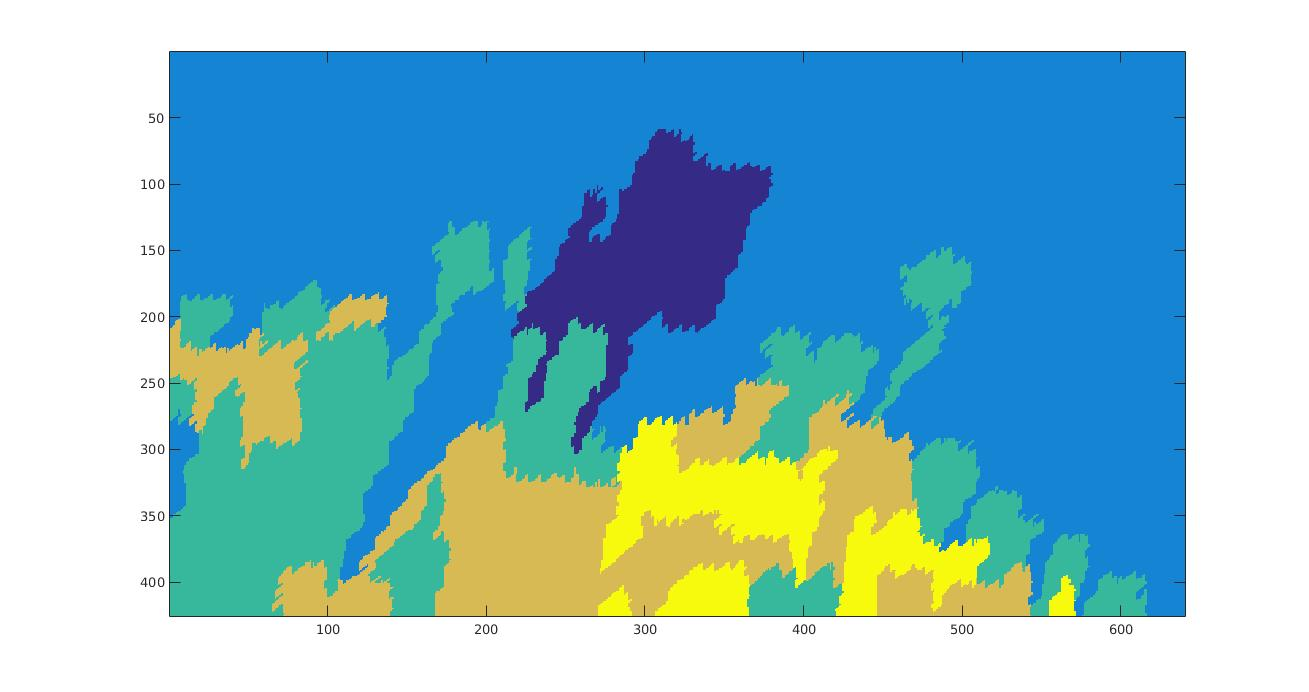
\includegraphics[width=\linewidth]{superpixel_rgb_mean/bee_5_500_20.jpg}
	 		\caption{superpixel level=500}
		\end{figure}
	\end{minipage}
	\hspace{0.05\linewidth}
	\begin{minipage}{0.45\linewidth}
			\begin{figure} [H]
				\centering
				 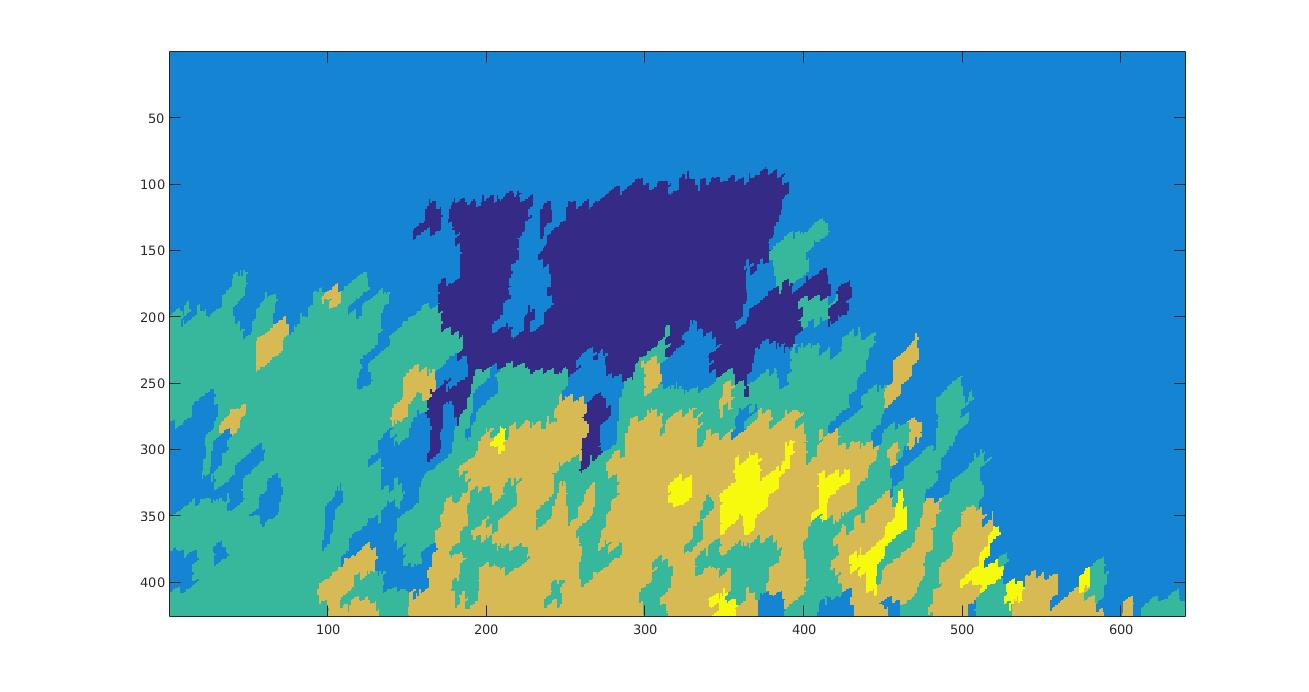
\includegraphics[width=\linewidth]{superpixel_rgb_mean/bee_5_2000_20.jpg}
	 			\caption{superpixel level=2000}
			\end{figure}
	\end{minipage}
	\hspace{0.05\linewidth}
	\begin{minipage}{0.45\linewidth}
		\begin{figure} [H]
			\centering
			 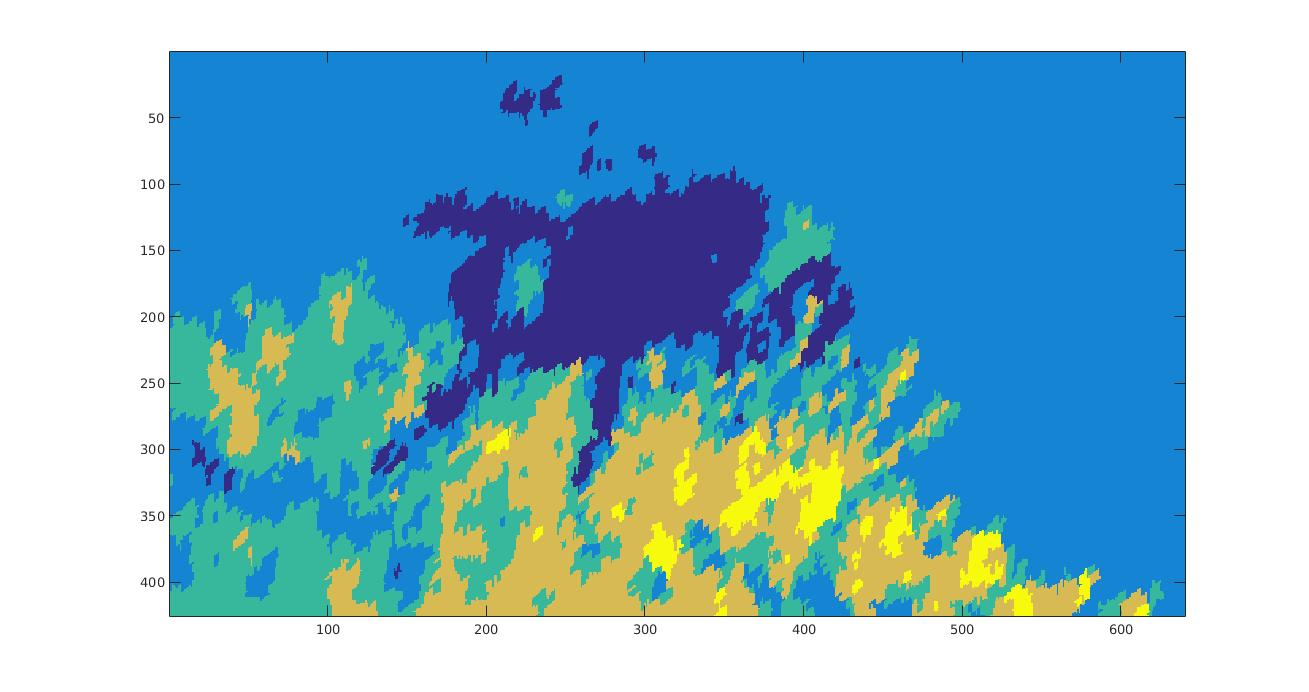
\includegraphics[width=\linewidth]{superpixel_rgb_mean/bee_5_5000_20.jpg}
	 		\caption{superpixel level=5000}
		\end{figure}
	\end{minipage}
\end{minipage}

\begin{minipage}{\linewidth}
\centering
	\textsc{\large Results for k=10;}\\[0.1 cm]  
	\begin{minipage}{0.45\linewidth}
		\begin{figure} [H]
			\centering
			 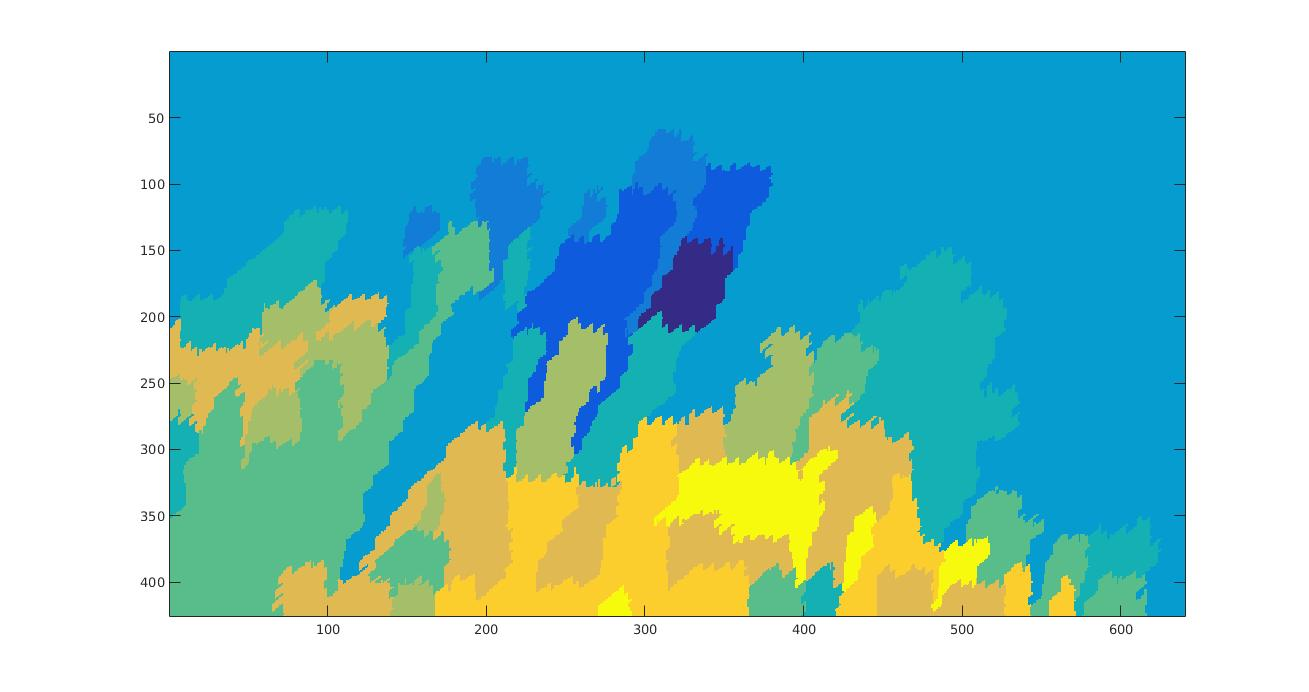
\includegraphics[width=\linewidth]{superpixel_rgb_mean/bee_10_500_20.jpg}
	 		\caption{superpixel level=500}
		\end{figure}
	\end{minipage}
	\hspace{0.05\linewidth}
	\begin{minipage}{0.45\linewidth}
			\begin{figure} [H]
				\centering
				 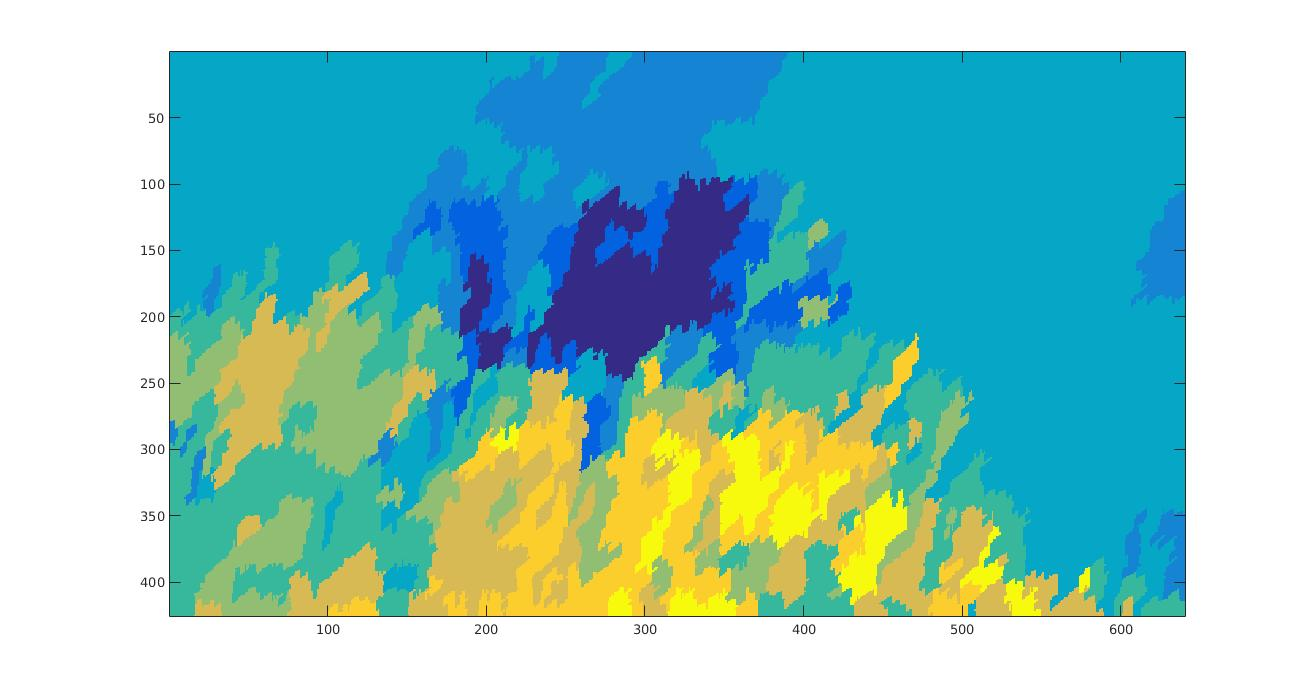
\includegraphics[width=\linewidth]{superpixel_rgb_mean/bee_10_2000_20.jpg}
	 			\caption{superpixel level=2000}
			\end{figure}
	\end{minipage}
	\hspace{0.05\linewidth}
	\begin{minipage}{0.45\linewidth}
		\begin{figure} [H]
			\centering
			 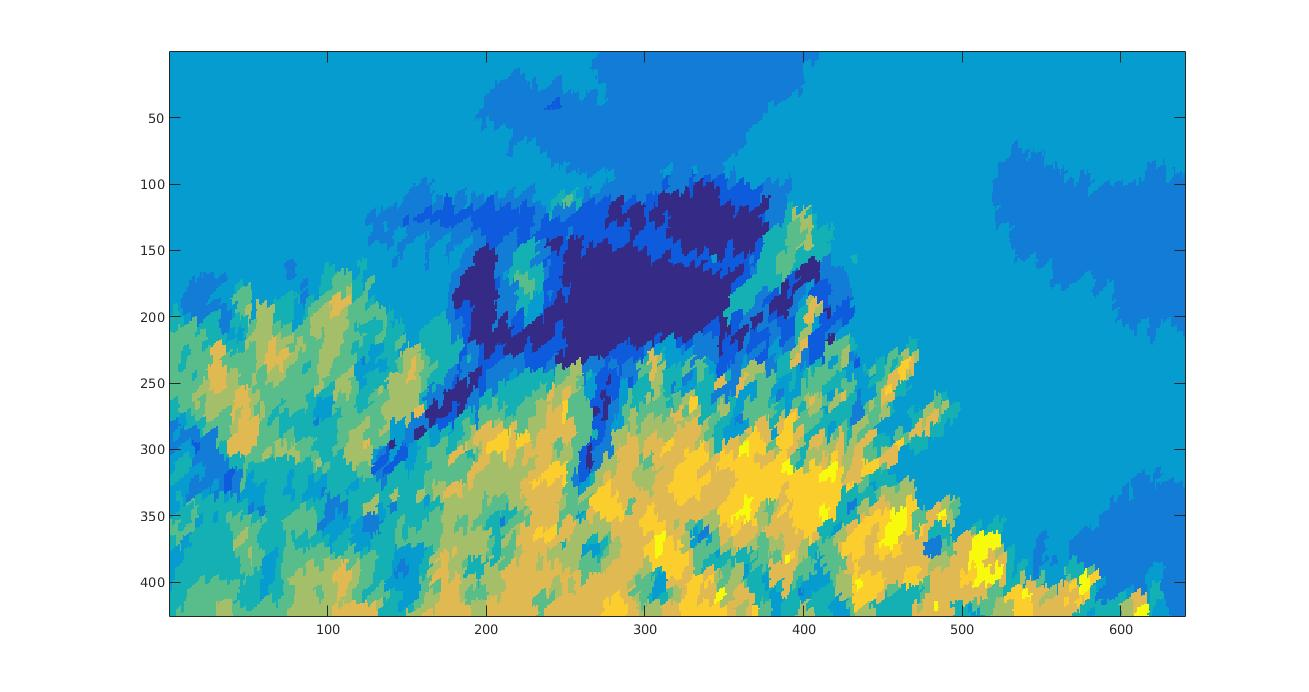
\includegraphics[width=\linewidth]{superpixel_rgb_mean/bee_10_5000_20.jpg}
	 		\caption{superpixel level=5000}
		\end{figure}
	\end{minipage}
\end{minipage}

\begin{minipage}{\linewidth}
\centering
	\textsc{\large Results for k=15;}\\[0.1 cm]  
	\begin{minipage}{0.45\linewidth}
		\begin{figure} [H]
			\centering
			 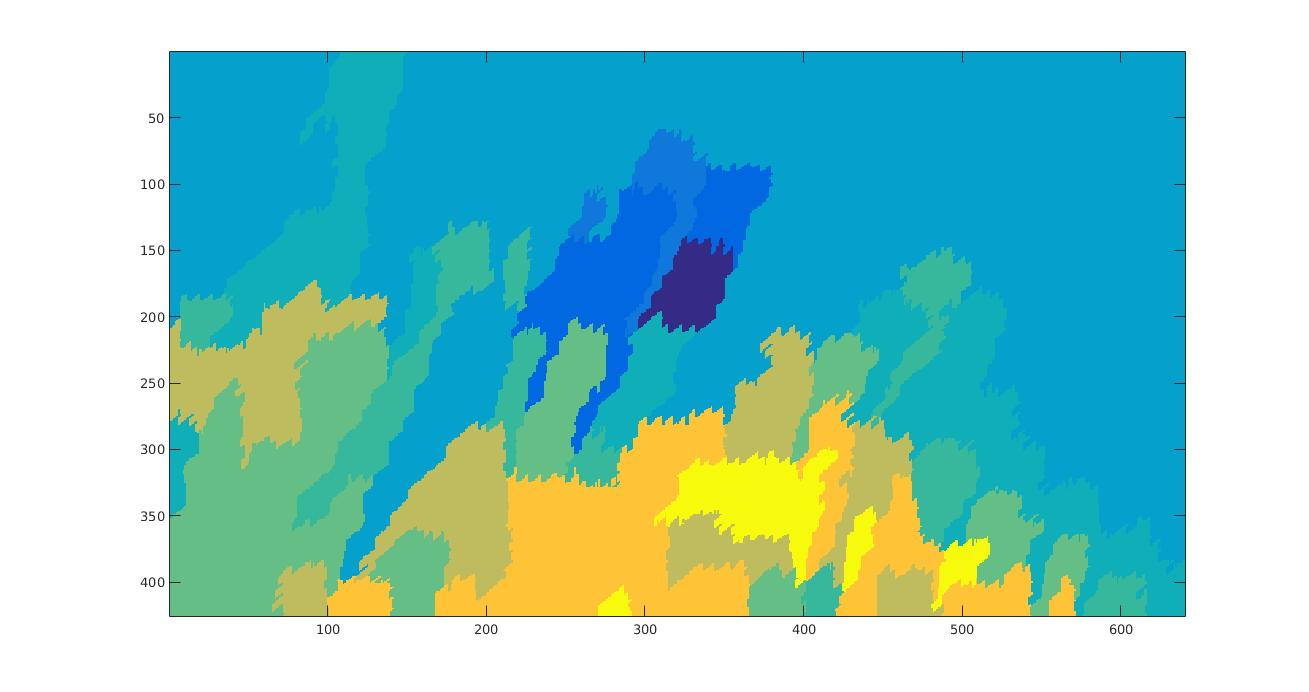
\includegraphics[width=\linewidth]{superpixel_rgb_mean/bee_15_500_20.jpg}
	 		\caption{superpixel level=500}
		\end{figure}
	\end{minipage}
	\hspace{0.05\linewidth}
	\begin{minipage}{0.45\linewidth}
			\begin{figure} [H]
				\centering
				 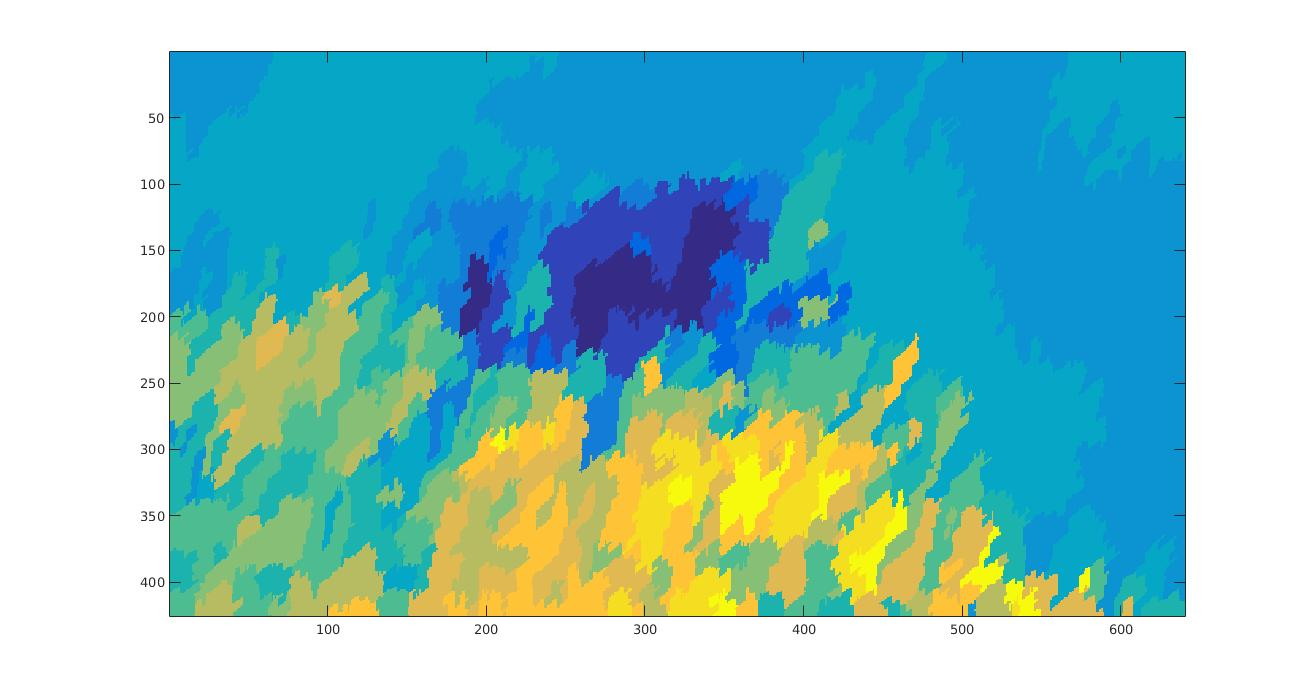
\includegraphics[width=\linewidth]{superpixel_rgb_mean/bee_15_2000_20.jpg}
	 			\caption{superpixel level=2000}
			\end{figure}
	\end{minipage}
	\hspace{0.05\linewidth}
	\begin{minipage}{0.45\linewidth}
		\begin{figure} [H]
			\centering
			 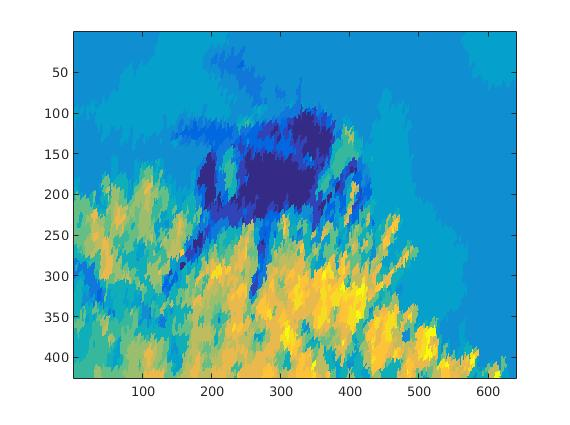
\includegraphics[width=\linewidth]{superpixel_rgb_mean/bee_15_5000_20.jpg}
	 		\caption{superpixel level=5000}
		\end{figure}
	\end{minipage}
\end{minipage}

\subsubsection*{RGB Color Histogram}

\subsubsection*{Mean Of Gabor Filter Responses}

\subsection{Effects of Parameters}
\paragraph{k parameter:} k parameter is defining the number of field.We are randomly choosing k point and trying to find the most close pixels for these point. When the definition of field is completed, for each field we are trying to find point of the mean of the field recursively. If we increase number of k, we can interested in less pixels because the fields have less size so we can see the image which has more details.

\paragraph{Superpixel level:} Superpixel is finding field that has same color. Superpixel level is the number of the field has same color. If we are using high superpixel level, it can be search field that has less size and it could be draw that has same color area for each superpixel.So super pixel level is giving the color information in image and high superpixel level has more detail than low superpixel level in color perception. We can see the results in Figure 3-6-9. When k is equal 5, 

\section{K-means Clustering}
K-means clustering is the easiest way to fix clustering problem. The main idea is to define k field, one for each cluster. 
\subsection*{Steps for K-means Clustering}
\begin{enumerate}
\item Randomly place K points into the space represented by the objects that are being clustered. These points represent initial group fields.
\item Assign each object to the group that has the closest field.
\item When all objects have been assigned, recalculate the positions of the K field.
\item Repeat Steps 2 and 3 until no more longer move..
\end{enumerate}
K-means function should be get two parameters(feature matrix, k). It should be generate k number of field. Then in the fields the mean should be changed recursively while it is same point for each field. It should be used for pixel-feature level features and superpixel-level features.
\subsection{Solution}


\subsubsection{Inputs Outputs}


\subsection{Effects of Parameters}
\paragraph{•}

\bibliographystyle{plain}
\bibliography{biblist}
  \begin{thebibliography}{1}
  \bibitem{1} \url{https://en.wikipedia.org/wiki/Pyramid_(image_processing)}
  \end{thebibliography}             
\end{document}


